\documentclass[a4paper,10pt]{article}
\usepackage{fullpage}
\usepackage{times}
\usepackage{listings}
\usepackage{xparse}
\usepackage{hyperref}
\usepackage{xcolor}
\usepackage{color}          % Code coloring
\usepackage[a4paper, margin=1in]{geometry}
\usepackage{minted}
\definecolor{mannibg}{HTML}{f0f3f3}
\setminted{frame=lines,linenos,framesep=7pt,bgcolor=mannibg,fontsize=\footnotesize}

\usepackage{graphicx}
\graphicspath{ {./images/} }
\usepackage{subcaption}

%\usepackage{subfig}
\usepackage[
backend=biber,
style=ieee,
sorting=ynt
]{biblatex}
\usepackage[
  hashEnumerators,
  definitionLists,
  footnotes,
  smartEllipses,
  tableCaptions,
  fencedCode,
  inlineFootnotes,
  citations,
  hybrid,
  html
]{markdown} 

\addbibresource{references.bib}
 
\usepackage{xcolor}
 
\definecolor{codegreen}{rgb}{0,0.6,0}
\definecolor{codegray}{rgb}{0.5,0.5,0.5}
\definecolor{codepurple}{rgb}{0.58,0,0.82}
\definecolor{backcolour}{rgb}{0.95,0.95,0.92}
 
\lstdefinestyle{mystyle}{
    backgroundcolor=\color{backcolour},   
    commentstyle=\color{codegreen},
    keywordstyle=\color{magenta},
    numberstyle=\tiny\color{codegray},
    stringstyle=\color{codepurple},
    basicstyle=\ttfamily\footnotesize,
    breakatwhitespace=false,         
    breaklines=true,                 
    captionpos=b,                    
    keepspaces=true,                 
    numbers=left,                    
    numbersep=5pt,                  
    showspaces=false,                
    showstringspaces=false,
    showtabs=false,                  
    tabsize=2
}
 
\lstset{style=mystyle}
\NewDocumentCommand{\codeword}{v}{%
\texttt{{#1}}%
}

\def\markdownOptionOutputDir{./build}

\iffalse
1. gather data from bb
2. run ./get_data.sh
3. run change clion deployment to remote
4. use jupyter locally
5. save everything
6. upload with ./upload_data_lib.sh
7. return to 1
\fi

\begin{document}

\title{L41: Lab 3 - The TCP State Machine, Latency, and Bandwidth}
\author{Nicolò Mazzucato \textless{}nm712\textgreater{}}
\date{\today}

\maketitle

\thispagestyle{empty}

\begin{abstract}           
   This experiment is about an investigation of the TCP protocol and its implementation in the FreeBSD operating system. Firstly, we compare the state machine described in the TCP specifications (RFC 793\cite{RFC793}) with the actual one in FreeBSD. Thanks to DUMMYNET, it is possible to witness and compare the behaviour of the TCP stack with different network latencies. Secondly, we investigate the effect of latency on bandwidth across time, analysing how the various congestion control techniques behave. We put particular attention into the comparison between automatic buffer resizing versus fixed size one.

   As a result, it is highlighted the connection between RTT (Round-Trip Time) and bandwidth.  Setting the size of socket buffers avoid expensive resizing on the way to the final bandwidth, resulting in the reach of a stable bandwidth in a faster way. The automatic socket buffer resizing policy makes the initial slow-start phase slower in all the tests. Since the congestion window is limited by the receiver available buffer size, with automatic buffer resizing the slow start phase increase is not exponential anymore and depends on the effective resizing policy. In the specific FreeBSD version used by the board, the buffer is incremented by small steps every time. While this gradual increase of the congestion window results in higher bandwidth for low latency, it is the main bottleneck to the speed of the slow start phase at higher latencies.
\end{abstract}

\iffalse
- state machine comparison with the RFC[] one manually setting differnet latencies (differences on the final sequence)
   - analysis of the flow-control and congestion control mechanisms, plotting graphs with the congestion window, and analysing how the tcp state variable change in time.
   - behaviour of auto-resizing sockets buffer
   - the connection between Latency, RTT and bandwidth

- [0,5,10,20,40] ms available
General todos:
- (-s = not automatic, but set)

generic things to write
- [x] write that the window advertisement is the space available in the receiver buffer.
- [x] receive window comparison
- [x] define RTT (and understand what it is)
- [x] write that the cwnd is calculated on duplicate ACKs
- [x] ssthreshould trimmed at the beginning
- [x] read chapter about TCP (chp. 14)
- [x] annotate trace with events from congestion control implementation
- [x] packet loss detection (draw something red when a packet loss is detected)
- [x] probe effect. Show the bandwidth graph with and without dtrace
- [x] retake data for overall bandwidth
- [x] add an indication for each duplicate ack in the graphs (packet loss)
- [x] write that there are too much things at 0ms and 5ms, that dtrace drops data (and try from cmd line to see if there is the message)
- [x] timeout with low latencies
- [x] gradual buffer increase more effective with low latencies? but why?
- [x] how to set socket buffer size
generic things to do 
- [.] Mark when  the different tcp phases begin (slowstart, congestion avoidance, fast recovery?) (use different colors in the graph)
- [x] understand if packet len is useful
- [x] profile to see what happens
- [-] packet size
- [-] graph with all the bandwidth
- [x] Add image of 0ms (or 5ms?) to justify why the overall bandwidth is higher.
- [x] write where the measurements are taken (which host)

generic things to investigate
- [x] why is the bandwidth higher with resizing buffers at small latencies
- [x] write about the dtrace buffer limitation
- [x] Explore the effects of socket-buffer limits and stack graph information on the flow-control versus congestion-control limits. How does socket-buffer auto-resizing help/hurt/not change performance? 
- [x] describe probe effect, if any?
- [x] dtrace precision problem; There are many timestamps that are the same:v (put this in limitations)
\fi

\clearpage

\setcounter{page}{1}

\section{Introduction}
The Transmission Control Protocol (TCP) is a protocol commonly used to exchange ordered, reliable and bi-directional streams of bytes over the IP protocol. Communication endpoints are identified by the couple (IP address) and (port number). 
TCP is implemented as a state machine due to the large number of cases to handle before, during, and after the data transfer. An initial "sync" between the two endpoints is called "three-way handshake". Its purpose is to exchange the sequence numbers and initialize all the kernel structures in the endpoints.
After this initial handshake, the connection is "established", where data can be exchanged.
The end of the connection requires another sequence of "FIN" packages to be exchanged by each endpoint. It can be initiated by one host, or by both at the same time. The latter option is compatible with high latency networks.

TCP packets go trough a network composed by many different intermediate devices, and it is nearly impossible to know in advance the available bandwidth. For this reason, TCP implements congestion control techniques to discover the maximum available bandwidth. This mechanism requires an initial phase where the transfer happens at reduced speed but depending on the network latency; it eventually converges to a speed near to real link available one.

\subsection{Congestion control}
The TCP congestion control takes into account two different factors: 
\begin{enumerate}
   \item The receiver available space. Each receiver operates with a finite amount of space to accommodate the data received. If this space ends, the receiver has to drop new packets. For this reason, in every ACK packet (sent from the receiver to the sender) the receiver inserts and advertised window size, based on the amount of space in the receive socket buffer. This variable is called 'Advertised window' from now on. 
   \item The effective network capacity. Every network link has a finite capacity. Trying to transmit more data than the network infrastructure could hold would result in packets loss. When the receiver has a gap in the sequence numbers (caused by a packet loss), it sends a duplicate ACK to hints the sender that the packet should be retransmitted. This influences the value of the congestion window, that is kept as a state variable on each side of the TCP connection, and it is changed according to three different phases (even if all the actual implementations might slightly differ).
\end{enumerate}
The congestion window change is handled in different phases, well described in the RFC 5681\cite{RFC_5681}:
\begin{itemize}
   \item Slow start. In this phase, the congestion window is increased by one MSS (Maximum Segment Size) for each acknowledgement received. This results in an exponential increase. However, this growth is limited by the advertised window: a limited advertised window might cause this phase to be all but exponential. Once congestion is detected (trough duplicate ACKs) the variable \codeword{ssthreshould} is set to half of the congestion window, and the slow start begins again. Once the congestion window reaches the "slow start threshold", the phase switches to congestion avoidance.
   \item Congestion avoidance. In this phase, there is a more cautious increase in the congestion window. The growth is not exponential anymore but aims to be linear. In the case of a timeout, the phase returns to slow start with a threshold half the congestion window.
   \item Fast recovery. This phase is entered once a duplicate ACK is received in either of the previous states. It allows resending the missing packet before waiting for the end of the retransmission timeout associated with it.
\end{itemize}
The TCP bandwidth is then dependent on the minimum between the receiver available buffer size, and the congestion window.

\section{Experimental setup and methodology}

\subsection{Hardware setup}

For the experiment, it is used the BeagleBone Black board with an open-source FreeBSD\cite{mckusick_design_2014} 11.0 operating system’s ARMv7 port. This board has the following characteristics:
\begin{itemize}
    \item 512MB DDR3 RAM
    \item 4GB 8-bit eMMC on-board flash storage
    \item AM335x 1GHz ARM® Cortex-A8 - Single core 32-bit processor\cite{noauthor_am3358_nodate}
    \begin{itemize}
        \item Independent 32KB L1 instructions and data cache
        \item Shared L2 cache (256KB)
        \item 64 bytes cache lines
    \end{itemize}
\end{itemize}

The board mounts an SD card. However, it is not relevant for the test, as the benchmark is in-memory.
      

\subsection {Methodology}
The benchmark consists of a program able to create two ends of a TCP socket over the loopback interface. The program is statically linked so that we can neglect dynamic linking performance overhead. The program opens a socket using the \codeword{socket(2)} system call, bind it to a specific port, and listen for new connections. The receiving end similarly opens a socket, and uses \codeword{connect(2)} to connect with the other endpoint at the same port. During the benchmark, a fixed size amount of data is transferred from the sender to the receiver. Afterwards, the \codeword{close(2)} system call initiates the closing phase.

The focus of this experiment is on the kernel socket buffer resizing policies. In particular, we compare two cases: the automatic resizing, and the fixed one.

We use \codeword{setsockopt()} to set the size of both the send (\codeword{SO_SNDBUF}) and receive (\codeword{SO_RCVBUF}) socket buffers to the buffer size we are using during the transfer.

IPFW, the firewall used, provides DUMMYNET\cite{luigirizzo_luigirizzodummynet_2020}, that allows traffic shaping. In this experiment, IPFW is used to generate two pipes and set the latency in each one of those. The RTT (Round-Trip Time) is the sum of the latencies (e.g. for 10 ms latencies, the RTT is 20ms). The pipes are used to filter the traffic, and selectively apply the delay only to the traffic we care about. We then generate the state transition graph at different levels of delays to see the differences.
The actors of the communication, in our case, are two threads: one that sends data, and the other that receives it. The dimension of the buffer passed to the \codeword{write(2)} system call is 128KB for the state-machine generation, and 1MB for the remaining graphs.
The total amount of data transferred is 16MB for each benchmark run.

The loopback Maximum Transmission Unit (MTU) is manually set to 1,500 bytes before each test. In this way, it is possible to avoid larger values that might have been caused to the local nature of the test, resembling real LAN or WAN results.

We use DTrace for most performance measurements. In particular, we use the following providers:

\begin{itemize}
   \item Function Boundary Tracing (FBT) provider. We are using probes on specific functions. There are also TCP generic ones, portable across different systems, but they do not provide the needed number of parameters to make all the analysis, and some of them (e.g. statically defined probes for buffer resizing) are missing. The output from the tracing of the entire kernel's function entry and exit point is then visualized into Perfetto\cite{noauthor_perfetto_nodate}, to inspect for further interesting behaviours graphically.
   \item Profile provider. It fires a probe at a given frequency. We use it to aggregate the results of \codeword{stack()} and see where most of the time is spent. 
\end{itemize}

After each benchmark run, two seconds have been added before stopping the DTrace instrumentation, to make sure to capture any final timing-related event. Without those, the state transition graphs were sometimes different: often the time-wait phase was not reached, because it was entered after the benchmark end when the DTrace instrumentation was not running anymore.

The verbose benchmark output, containing the IPC loop duration measured from the program and printed to stdout, is then used to evaluate the probe-effect caused by DTrace.


All the benchmark runs are executed 11 times for each parameter value, dropping the first one. In each graph, it is possible to see the error as a vertical line. However, in almost all cases, this error is negligible, highlighting a controlled benchmarking environment. The value on the graphs is the median of the 10 measurements.

While the DTrace instrumentation covers both sender and receiver, the graphs only contain value from the sender. In the case of bandwidth measurements, we use the timestamps and ACK to give a rought estimate. In the other cases, packets are filtered by destination port.

\subsection{Limitations}

During the tracing, several other processes were running, and this might have slighly influenced the results. In particular:
\begin{itemize}
    \item One ssh session
    \item A Jupyter notebook
\end{itemize}

In addition, due to the limited computational power of the board, the frequency of the DTrace profile provider had to be limited to under 30Hz, with system instability error messages at higher frequencies, expecially at low latency values.

\section{Results and discussion}

\subsection{TCP state-transition diagram}
%overall figures
\begin{figure}[]
\begin{subfigure}{.30\textwidth}
    \centering
    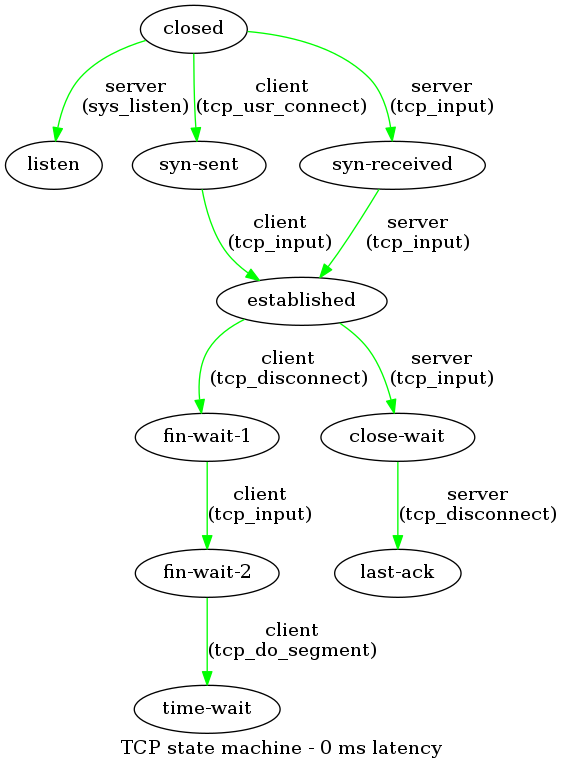
\includegraphics[width=\textwidth]{images/TCP_state_machine_0_ms.png}
    \caption{TCP state transition graph with 0ms latency.}
    \label{fig:0ms_latency}
\end{subfigure}%
\qquad
\begin{subfigure}{.30\textwidth}
   \centering
   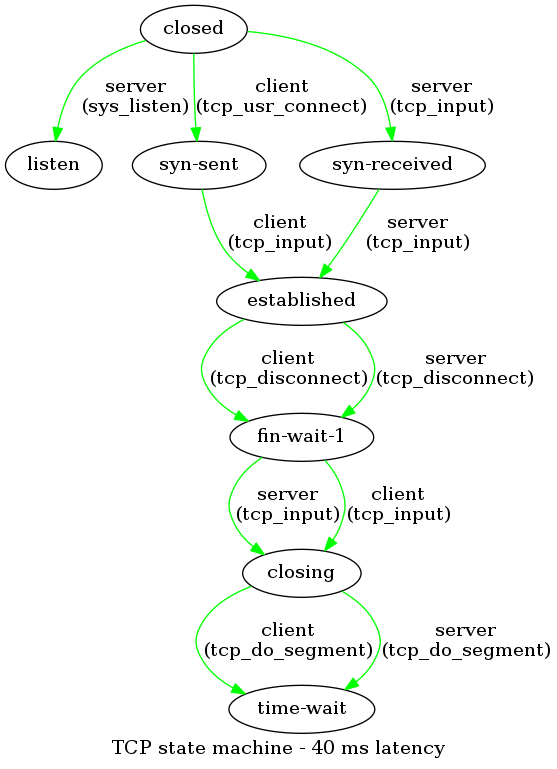
\includegraphics[width=\textwidth]{images/TCP_state_machine_40_ms.png}
    \caption{TCP state transition graph with 40ms latency.}
    \label{fig:40ms_latency}
\end{subfigure}
\qquad
\begin{subfigure}{.30\textwidth}
   \centering
   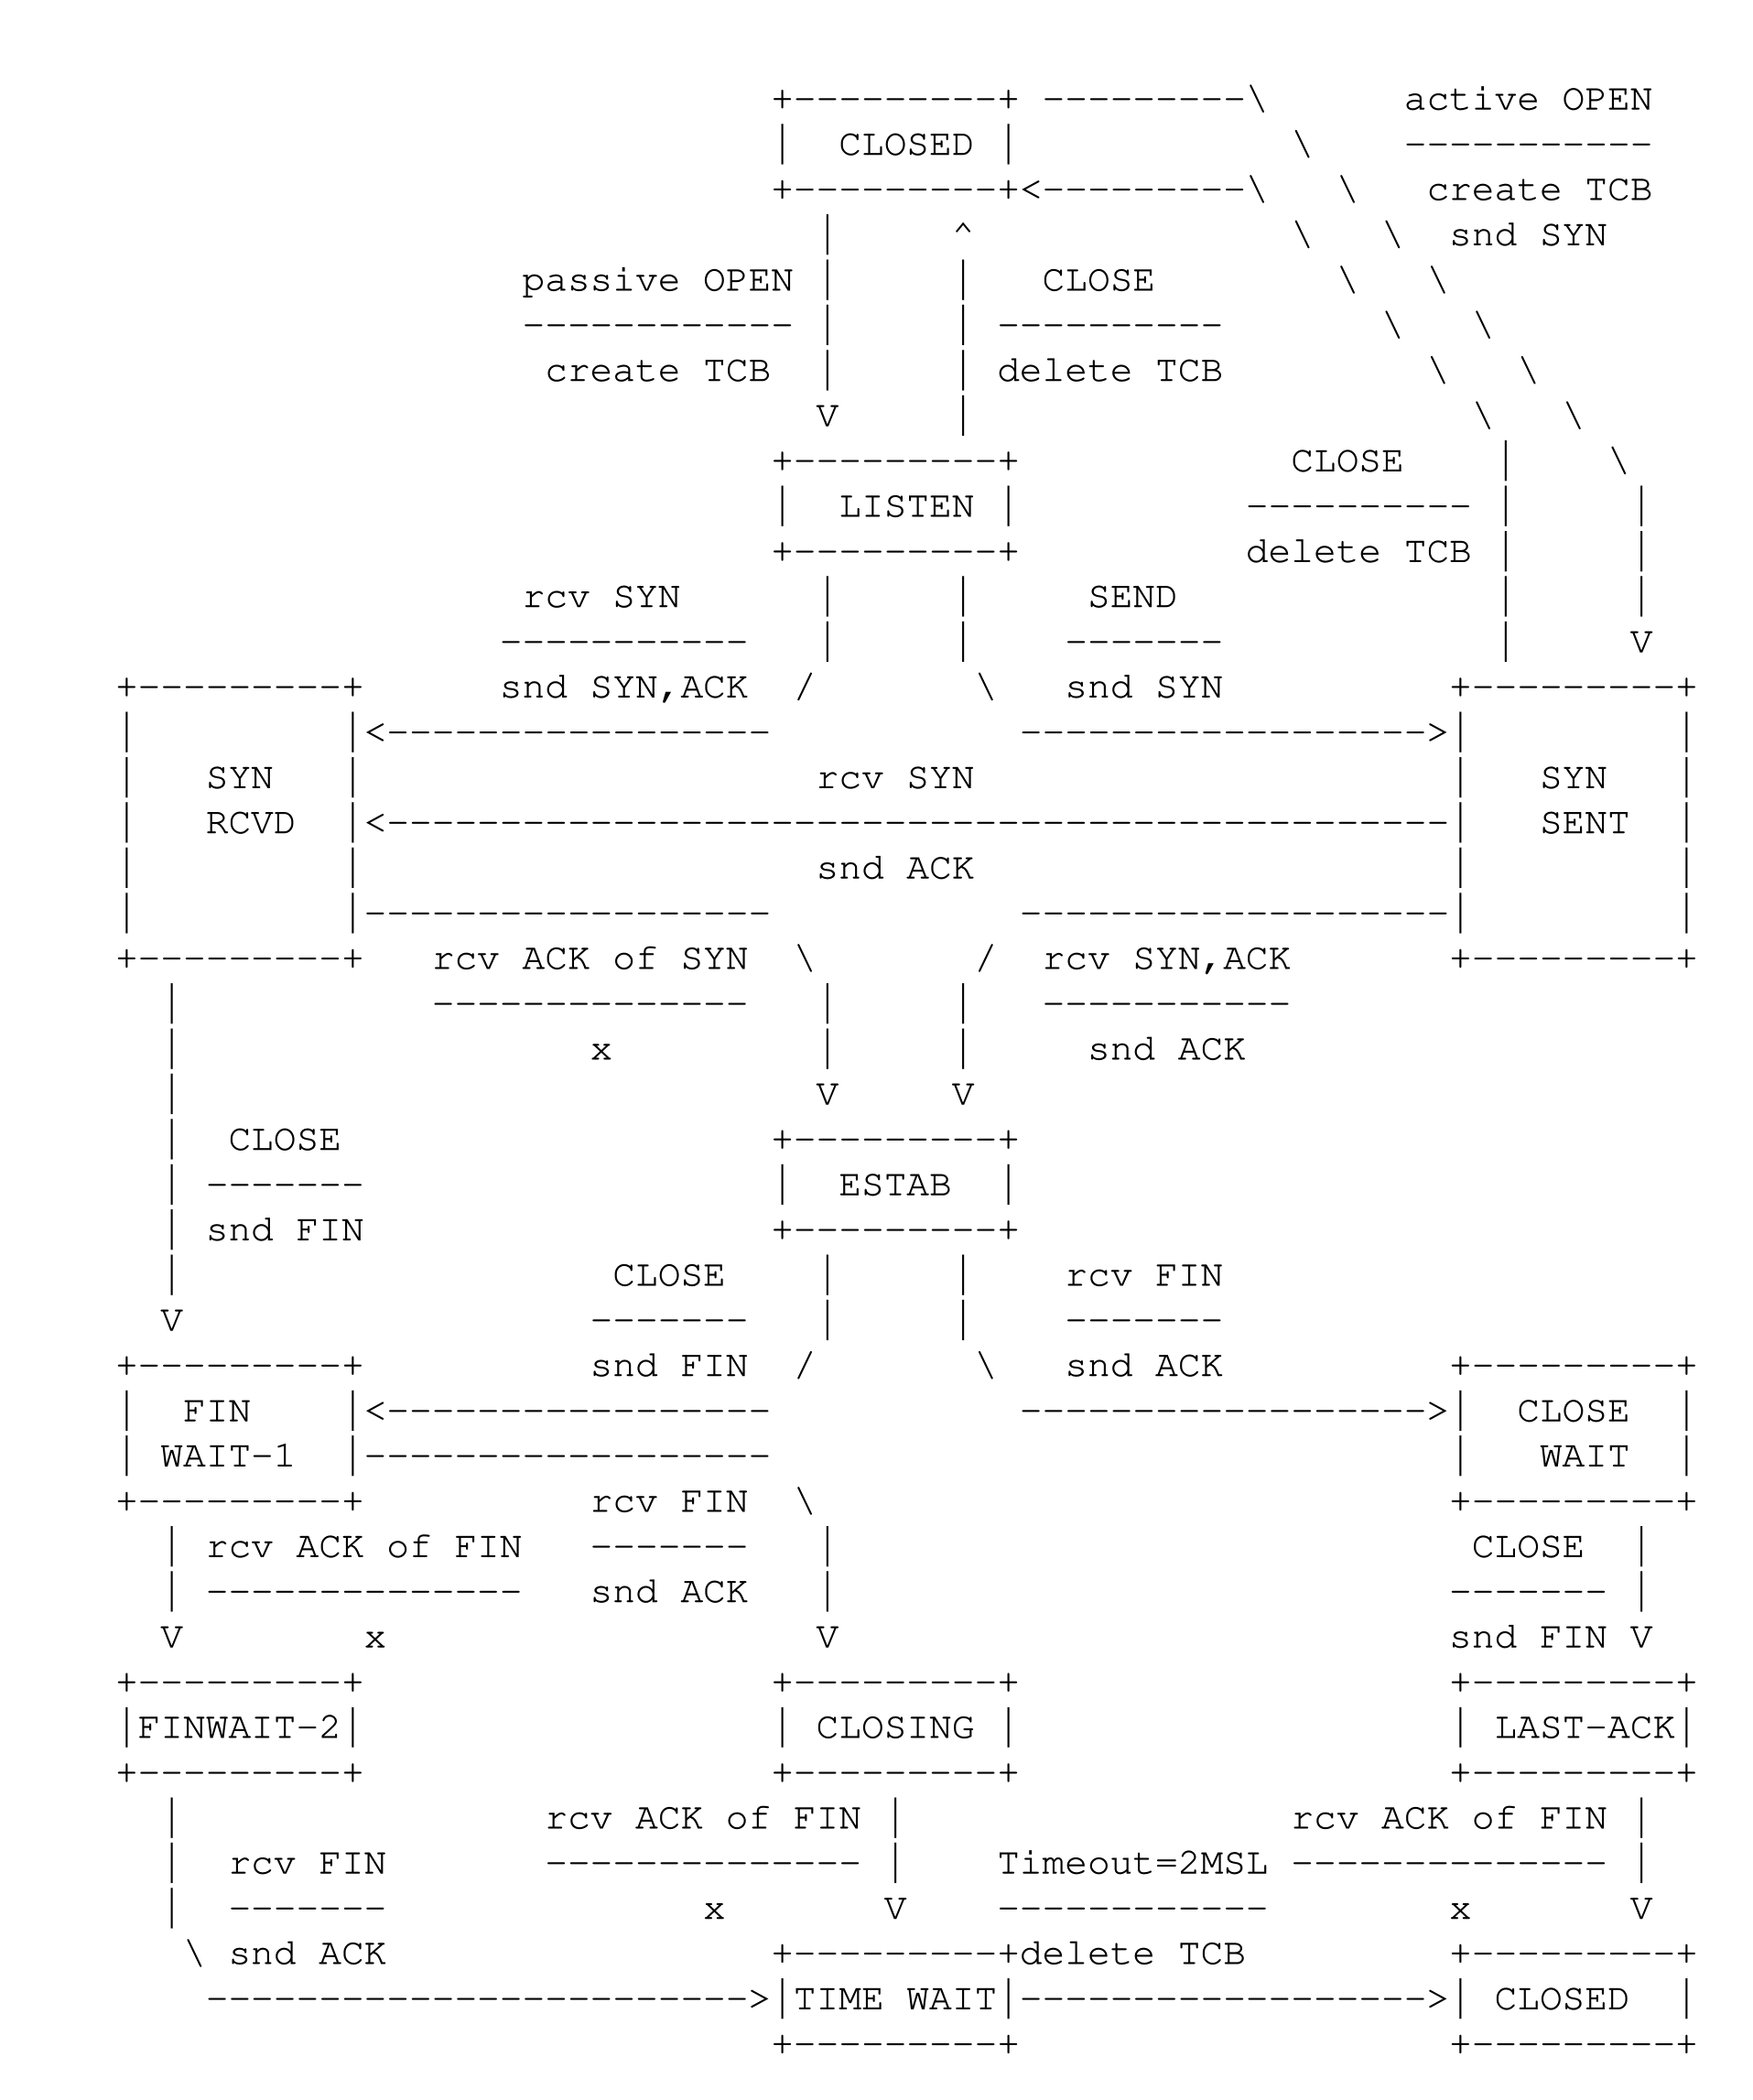
\includegraphics[width=\textwidth]{images/RFC_Graph.png}
    \caption{TCP state transition according to RFC 793.}
    \label{fig:RFC_graph}
\end{subfigure}
\caption[short]{Comparison between measured state transitions and RFC 793.}
\end{figure}

We generated TCP state transition graphs with different latency values, from 0ms to 40ms, with 5ms steps. It is possible to notice that from a latency value of 10ms there is a slighly different shape in the connection closing phase. In particular:
\begin{itemize}
   \item With 0 ms latency, as shown in figure \ref{fig:0ms_latency}, the close phase of the connection goes through the \codeword{fin-wait-1} and \codeword{fin-wait-2} states (client side)
   \item From a latency of 10ms onwards, as shown in figure \ref{fig:40ms_latency}, both the server and the client reach the \codeword{fin-wait-1} state, but then they both enter into the closing state, without passing through the \codeword{fin-wait-2} state.
\end{itemize}

This behaviour is clearly explained in the RFC 793\cite{RFC793} on page 42. In the former case, it happens that the server sends the close packet (with the \codeword{FIN}), then the client receives it before closing the connection itself.
In the latter case, we have that due to the latency, the connection is closed simultaneously by both actors. None of them receives the other FIN before sending its own FIN is sent. For this reason, they both switch to fin-wait-1. When they receive each other FIN, they switch to closing, and after having received the ACK of the FIN, they go to the time-wait state.

There is another small difference between the generated graph and the RFC one. The server, does not transition from listen to \codeword{syn-received}, but from closed to \codeword{syn-receive}. In the RFC graph, there are other transitions not performed during the benchmark, related to cases such as the closing of a connection before the proper establishment.

% todo probe effect? in this case not relevant I think, but how to mseasure it? probably overall time at each delay level?


\subsection{TCP variables across time}
\label{sec:tcp_variables}


\begin{figure}[]
\begin{subfigure}{\textwidth}
    \centering
    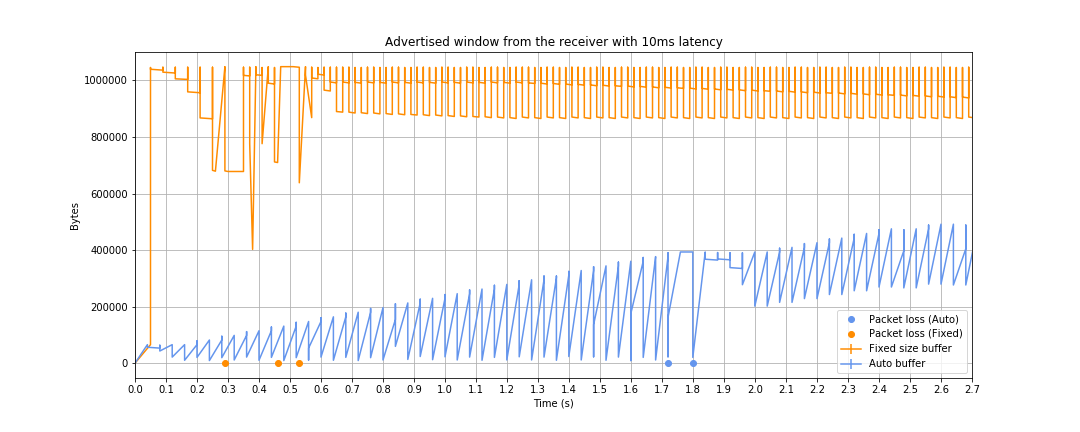
\includegraphics[width=\textwidth]{images/10_wnd_comparison.png}
    \caption{Receiver available space sent trough ACK across time.}
    \label{fig:10ms_wnd}
\end{subfigure}%
\qquad
\begin{subfigure}{\textwidth}
   \centering
   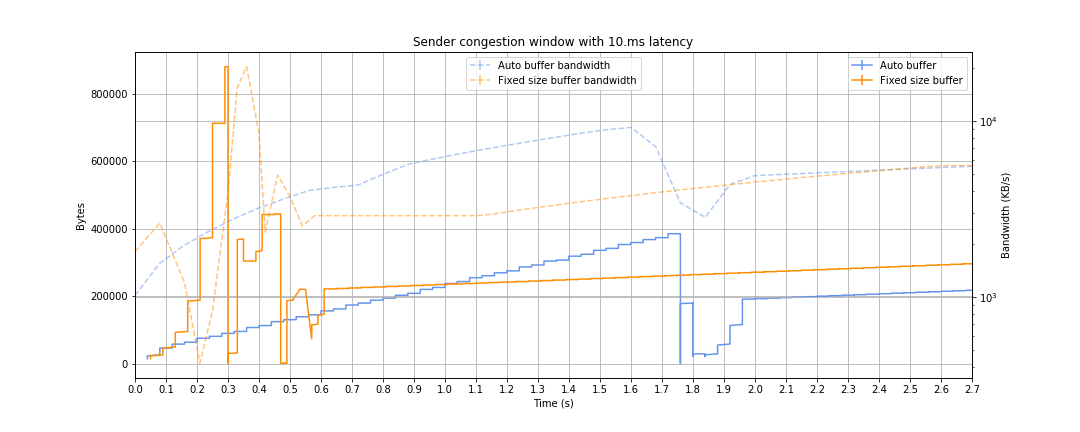
\includegraphics[width=\textwidth]{images/10_cwnd_w_bandwidth.png}
    \caption{TCP congestion window across time, with bandwidth.}
    \label{fig:10ms_cwnd}
\end{subfigure}
\qquad
\begin{subfigure}{0.5\textwidth}
   \centering
   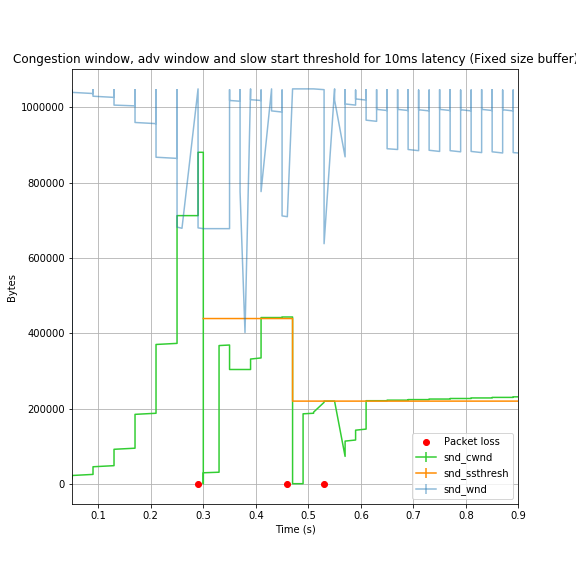
\includegraphics[width=\textwidth]{images/10_detail_windows_fixed.png}
   \caption{TCP congestion windows for fixed size buffers.}
    \label{fig:10ms_fixed}
\end{subfigure}
\qquad
\begin{subfigure}{0.5\textwidth}
   \centering
   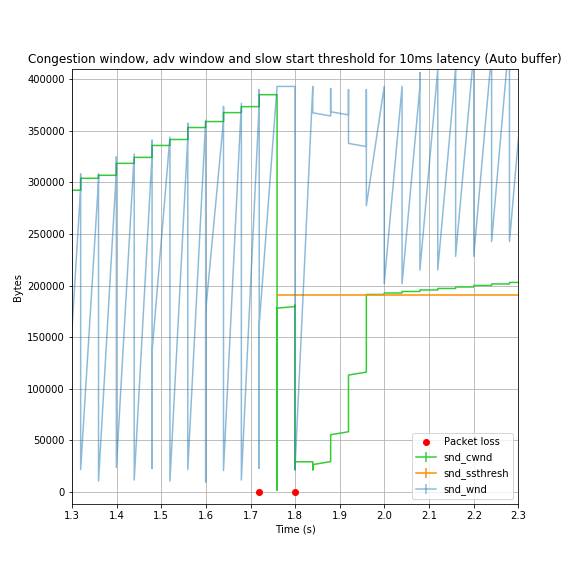
\includegraphics[width=\textwidth]{images/10_detail_windows_auto.png}
    \caption{TCP congestion windows for automatic resizing buffer.}
    \label{fig:10ms_auto}
\end{subfigure}

\caption[short]{TCP variables comparison during 10 ms latency transfer}
\label{fig:tcp_variables}
\end{figure}

Figure \ref{fig:tcp_variables} compares the various TCP variables in the case of auto-resize and fixed buffers with a latency set to 10ms. This value of latency, as shown in the probe effect evaluation, does not have an high overhead caused by DTrace. Those graphs can help to understand the differences in the bandwidth achieved at the various latencies, displayed in figure \ref{fig:bandwidth}. 

Figure \ref{fig:10ms_wnd} shows the advertised available buffer size in the receiver. From the comparison between the two buffer sizing policies, it is clear that the fixed-size one oversizes the buffer. The bandwidth never allows having more than half of it filled. During the initial slow-start phase, it can be seen how the buffer gets filled fastly. Afterwards, the available space always remains above 8 MB. However, as an effect of bandwidth increase over time, it is possible to see how the buffer gets filled more at every period from 0.6 seconds afterwards. As a consequence of the oversizing, the available space is never a limiting factor for the connection speed in this instance. 
On the other side, the automatically resized one has a more cautious approach: the initial buffer sizes seems to increase slowly with time. An available receiving buffer size near to 0 is often reached. After each one of those events, the buffer size seems to increase slightly. Up until 1.8s, the receiver buffer size is the limiting factor for the overall bandwidth. 

Figure \ref{fig:10ms_cwnd} shows the congestion window progress over time, with an overlay of the bandwidth. It is clear how the congestion window and the measured bandwidth are highly correlated. However, bandwidth dashed lines are the results of smoothing, and useful only as a general indication. In the slow start phase, two different progression strategies are adopted based on the buffer resizing policy. For fixed-size buffers, the congestion window increase is exponential, with a doubling at each step until a packet loss is witnessed. On the other hand, with an automatic resizing policy, the congestion window has a more linear increase, that takes more time to reach a packet loss. Once this happens, a new exponential increase is entered, until the slow start threshold is reached.
In both cases, when the slow start threshold is met, it is possible to see the linear growth of the congestion avoidance phase, where the congestion window is slowly increased by one segment size every RTT.

In figures \ref{fig:10ms_auto} and \ref{fig:10ms_fixed} we can compare what happens before and after the loss of a packet, and explain the reason why the increase is exponential in the fixed-sized case, and almost linear in the automatic buffer resizing case. 
The packet losses have been identified by an ACK received three times from the sender. 
Regarding the automatically sized buffer case, figure \ref{fig:10ms_auto}, it is possible to notice that the limiting factor before the packet loss was the receiver available size. The congestion window never increases above the receiver maximum available buffer size. After the packet loss (identified by the red dot), the slow start threshold is lowered to half the congestion window (in green in the graph). The first part of the slow start threshold (before the packet loss), is not displayed in the graph and can be considerate arbitrarily high. However, soon after (at second 1.8) the receiver buffer returns to limit its increase (for the last time). Afterwards, the receiver buffer is not a limiting factor anymore so that the congestion window can proceed with the exponential growth.
An explanation of the extremely high growth in figure \ref{fig:10ms_auto} between the two packet loss is that a high number of acknowledgements received in a short amount of time: each one of them increased the congestion window by one MSS.


\begin{figure}[]
\centering
\begin{subfigure}{0.8\textwidth}
    \centering
    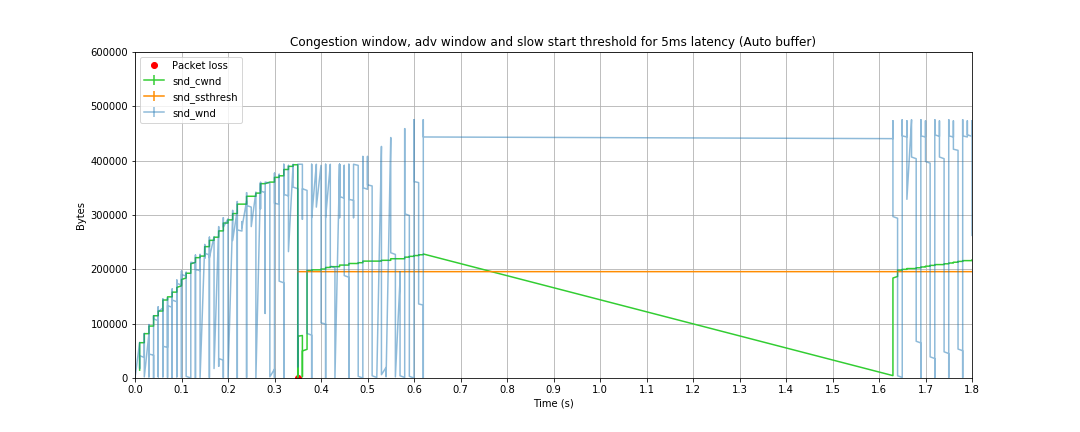
\includegraphics[width=\textwidth]{images/5_cwnd_wnd_comparison_auto.png}
    \caption{TCP windows during a transfer size with 5ms latency, automatic buffer resizing}
    \label{fig:5ms_wnd_auto}
\end{subfigure}%
\qquad
\centering
\begin{subfigure}{0.8\textwidth}
   \centering
   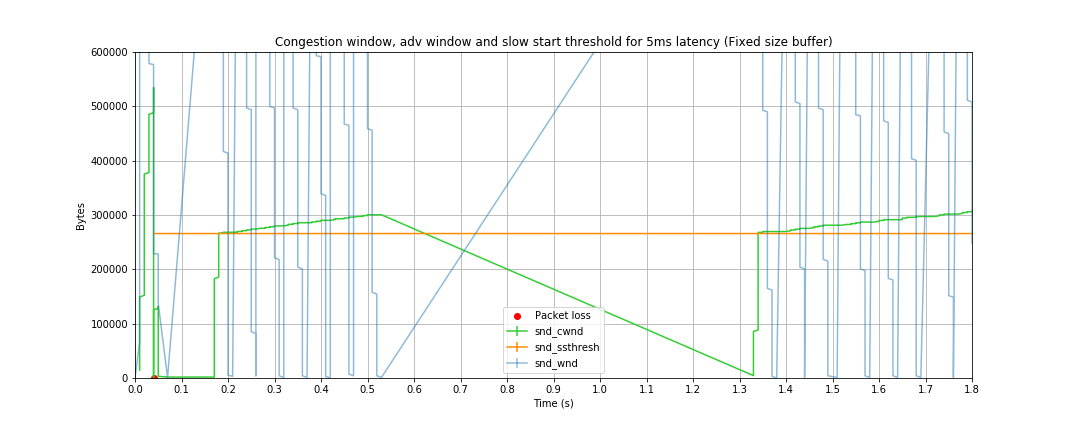
\includegraphics[width=\textwidth]{images/5_cwnd_wnd_comparison_fixed.png}
   \caption{TCP windows during a transfer size with 5ms latency, fixed buffer size}
   \label{fig:5ms_wnd_fixed}
\end{subfigure}
\caption[short]{TCP variables comparison during 5 ms latency transfer}
\label{fig:tcp_variables_5ms}
\end{figure}


It is interesting to notice what happens with a latency of 5ms, as shown in figure \ref{fig:tcp_variables_5ms}. Here, the scale of the x and y-axis is the same, even if the duration of the transfer is different. As figure \ref{fig:bandwidth} shows, up until 5ms, the bandwidth of the automatic buffer resizing is higher. 
Analyzing figure \ref{fig:5ms_wnd_fixed}, representing the fixed buffer size case, we can notice how the slow start phase spikes immediately, resulting in a slow-start threshold much higher than the automatic buffer case in figure \ref{fig:5ms_wnd_auto}. Soon after the packet loss is reached, we can see how the congestion window remains at zero for more than 100 milliseconds. The reason is likely to be a timer in the sender. The sender might not have received an ACK for a packet.
On the other side, the automatic buffer case maintains a slower growth rate in the slow start phase, that allows the exchange of more data before starting the congestion avoidance phase. In both cases, we can notice a long gap after the first congestion avoidance phase. Since no packet loss resulting in three different acknowledgements is displayed in the graph, it is likely generated by a timer in the sender: the receiver was not able to receive any packages from a point forward, nor it was not able to signal the packets loss.
However, the faster result of the automatic buffer case has been accomplished only because of the limited size of data exchanged: the slow start threshold is higher in the fixed-sized buffer, so the final bandwidth during the congestion avoidance phase is higher as well.
\subsection{FreeBSD automatic resize policy}

\begin{markdown}
Looking into the buffer resizing policy of the OS might help to explain the behaviours recorded. From figure \ref{fig:10ms_wnd} it is clear that the resizing happens by adding a constant step to the current buffer size. The FreeBSD 11 code confirms this. From \cite{tcp\_input} it is possible to see that the variable `tcp_autorcvbuf_inc` is defined as:
~~~c
VNET_DEFINE(int, tcp_autorcvbuf_inc) = 16*1024;
// ...
VNET_DEFINE(int, tcp_autorcvbuf_max) = 2*1024*1024;
~~~
And then, later, in `tcp_autorcvbuf` it is used to compute the new size:
~~~c
newsize = min(so->so_rcv.sb_hiwat +
          V_tcp_autorcvbuf_inc, V_tcp_autorcvbuf_max);
~~~
However, in new versions of FreeBSD, the resizing policy is different. As an example, in the current FreeBSD 13, the policy is the following:
~~~c
newsize = min((so->so_rcv.sb_hiwat + (so->so_rcv.sb_hiwat/2)), V_tcp_autorcvbuf_max);
~~~
In this case, the new buffer size will be the actual one, plus half itself.
With this new buffer resizing policy, our results might have been different, with a smaller gap between the two policies at higher latencies.
\end{markdown}

\subsection{Bandwidth for each imposed latency}

\begin{figure}[h]
\centering
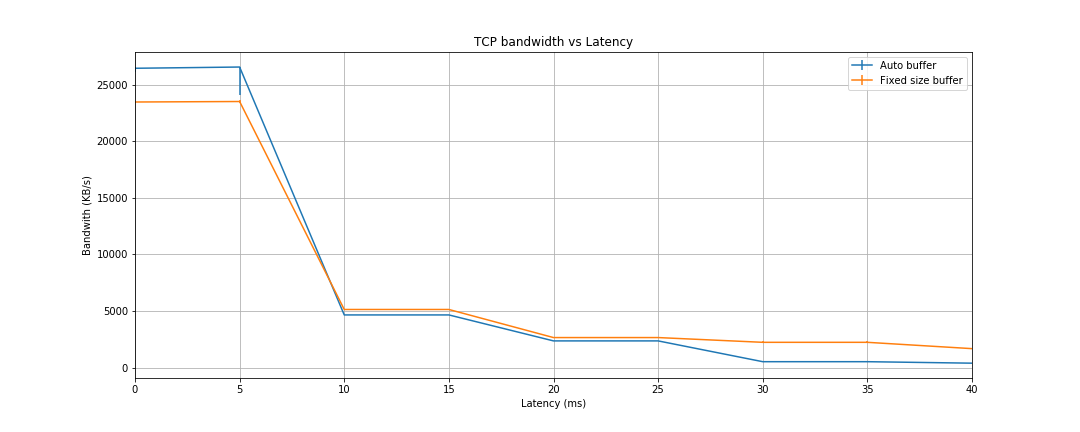
\includegraphics[width=\textwidth]{images/tcp_bandwidth.png}
  \caption{Imposed DUMMYNET lantecy vs bandwidth, both with and without socket-buffer auto-resizing}
   \label{fig:bandwidth}
\end{figure}

Figure \ref{fig:bandwidth} shows the bandwidth versus the DUMMYNET-imposed latency. We can notice that the bandwidth decrease is not linear. It remains almost constant until a latency of 5ms, when if suddenly drops at 10ms. At 20ms, it halves again, to then stay stationary from 30ms onwards.
The socket-buffer auto-resizing does not always result in a performance increase. We can notice different phases:
\begin{itemize}
   \item With low latencies, until 5ms, the auto-resizing policy allows a higher bandwidth. % todo write the reason.

   \item From a latency of 10ms, the overall bandwidth drops steadily. From 10ms to 25ms, the benchmark with statically sized buffers is always slightly faster than the other one, but comparable.
   \item From 30ms onwards the statically sized one allows a bandwidth more than double the auto-sized one. %todo because slow start doesn't gor as fast as the other
\end{itemize}

There are multiple reasons for this trend. 
An increased latency limits the congestion window growth rate, and as a consequence, the overall bandwidth, because the final transfer rate is reached more slowly. In our case, we are exchanging only 16 MB of data. As it is possible to see from figure\ref{fig:40_cwnd}, at high latencies TCP is not able to exit from the slow start phase, so it did not already find the full bandwidth available.
Also, The buffer slow growth rate limits the slow start growth even more.


\begin{figure}[h]
\centering
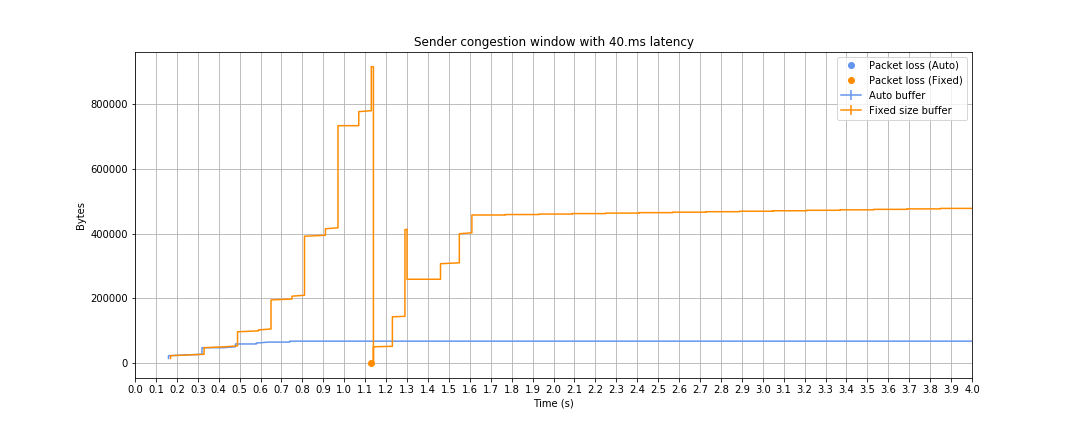
\includegraphics[width=\textwidth]{images/40_cwnd_comparison.png}
\caption{Congestion window with an imposed latency of 40ms. It is possible to notice how, with fixed size buffers, the slow start never finishes.}
\label{fig:40_cwnd}
\end{figure}

\subsection{Probe effect}

To indicate the performance overhead caused by DTrace, and understand if this overhead might have biased our result, we use the verbose benchmark output. In this mode, the measured transfer loop time is printed to stdout. The benchmark is executed for each latency value with and without the DTrace instrumentation running. Even if it does not provide a measurement as precise as the DTrace one, it gives a clear indication of the probes effect.
In particular, it is used the DTrace script that prints all the data when a packet is received, ignoring the DTrace output, and only gathering the stdout of the benchmark.
\begin{figure}[]
\begin{subfigure}{0.5\textwidth}
   \centering
   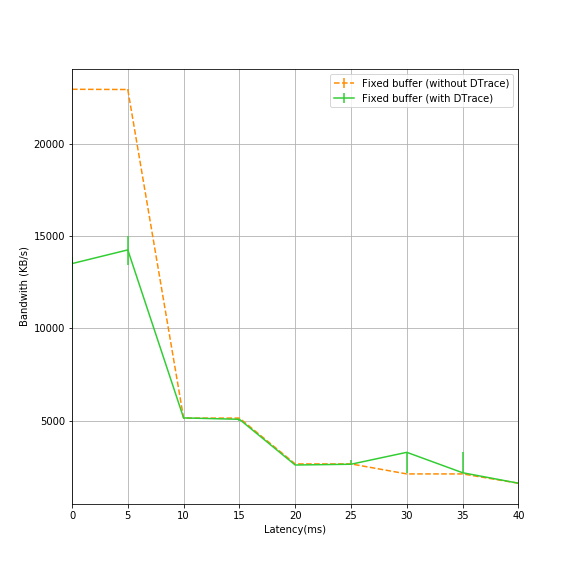
\includegraphics[width=\textwidth]{images/fixed_probe_effect.png}
   \caption{Probe effect for fixed buffers}
   \label{fig:fixed_probe}
\end{subfigure}
\qquad
\begin{subfigure}{0.5\textwidth}
   \centering
   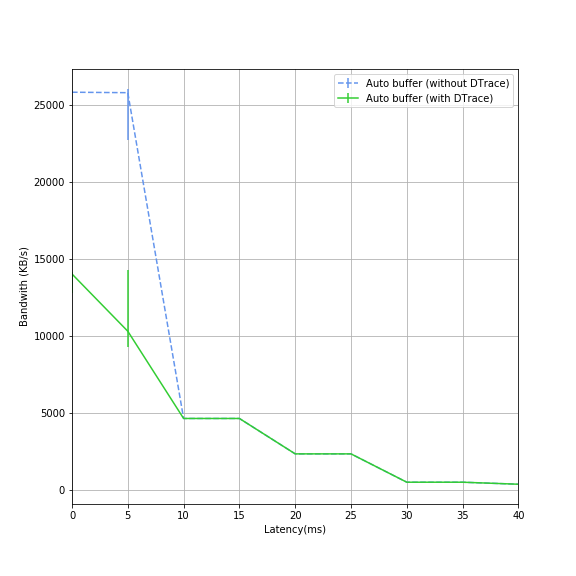
\includegraphics[width=\textwidth]{images/auto_probe_effect.png}
    \caption{Probe effect for automatic buffers}
    \label{fig:auto_probe}
\end{subfigure}

\caption[short]{Bandwidth comparison with and without DTrace instrumentation enabled}
\label{fig:probe_effect}
\end{figure}

As we can see from figures \ref{fig:fixed_probe} and \ref{fig:auto_probe}, the instrumentation performance overhead is significant with low latencies, but nearly negligible with latency values starting from 10 milliseconds. We can explain this with the high bandwidth achieved at low latencies, and as a consequence, TCP packets exchanged at this latency. This justifies the choice to do a detailed analysis of an instance of transfer at 10ms. From the evidence, the probe effect is not worth considering in section \ref{sec:tcp_variables}.

It is possible to notice a high variability in the measurements with DTrace instrumentation active, especially with fixed buffer sizes. A potential cause might be that the big fixed socket buffer uses most of the space available in the kernel, and the buffers used by DTrace to process the output are smaller, causing a different flushing policy that sometimes results in increased bandwidth.

Regarding the analysis of the state machine transitions, the probes fired a minimal amount of times (one for every edge in each graph), and it is unlikely that they changed the result in any way. As a comparison, the output of DTrace in the creation of the state transition graph always counts less than 15 lines (so, 15 probes activations). The output of all the variables when a packet is received always counts more than 140.000 lines (and probe invocations).


\section{Conclusions}

In conclusion, we have verified that the FreeBSD TCP state machine implementation follows the specifications described in the RFC 793\cite{RFC793}, and witnessed the closing behaviour in the presence of various values of latency.

The relationship between round-trip latency and bandwidth has been proven not linear in either buffer resizing policy cases. The reasons can be found in the effect of latencies in the TCP congestion window growth. An increased latency slows down the discovery of the link bandwidth. 

Socket-buffer auto-resizing has been proven useful with small latencies (less than 10ms). The reason is that the slower slow-start phase results in a higher congestion window for more time compared to the fixed buffer case, that started the congestion avoidance phase earlier, as can be seen from figure \ref{fig:tcp_variables_5ms}.
However,  at higher latencies, the slow buffer growth rate is the limiting factor for the slow start phase, limiting the congestion window increase, impeding to achieve an exponential growth rate in the initial phase (figure \ref{fig:40_cwnd}).  
All the benchmark executed at higher latencies are strongly affected by the fact that the initial slow-start phase did not finish. With the transfer of more data and another resizing policy such as the new FreeBSD 13 one, it is reasonable to expect a smaller gap between the final bandwidth at each latency value.

\newpage

\section{References}

\printbibliography

%\section{Appendices}


\end{document}
